\chapter{Social Tagging}\label{chap:social_tagging}

The massive expansion experienced by the Internet and web communities in the last decades has undoubtedly had a large effect on how we live our lives.

Today, we have access to many kinds of services on the web, such as search engines, email messaging, online purchases, and so on.

However, some of the most widely used websites are places where people interact with digital resources and with other human beings. Among these we could cite websites such as Facebook, Twitter, Youtube, StackOverflow, Quora, LinkedIn, Reddit, Sina Weibo and many others.

These online communities form what is commonly referred to \textit{social media} or \textit{social networking services}, or SNSs. \citep{obar_wildman_2015,hamburger_etal_2017}

Moreover, some of these so-called social media services support \textit{tags}, which are user-given, generally free-form, keywords used to help categorize resources \cite{mathes_2004}. These systems are called \textbf{Social Tagging Systems} or \textbf{STS}s.

We will go into more detail about these concepts, as well as some related terms (such as folksonomies) in the next sections.

\section{Examples of Social Tagging Systems}

Examples of STSs abound in the modern Web. We will present two different examples so that the reader can better grasp what a Social Tagging System looks like in practice.

\subsection{MovieLens}

MovieLens \footnote{https://movielens.org} is a research website run by GroupLens Research at the University of Minessota.

It provides users with personalized movie recommendations based on how they have rated individual films. In addition to information and ratings for many movies, MovieLens also lets users add tags to movies and view tags others have assigned.

As can be seen in the following image, tags allow users to give objective (\textit{car chase, espionage}) and subjective (\textit{great plot} attributes to resources, in this case films.

\begin{figure}[H]
    \centering
    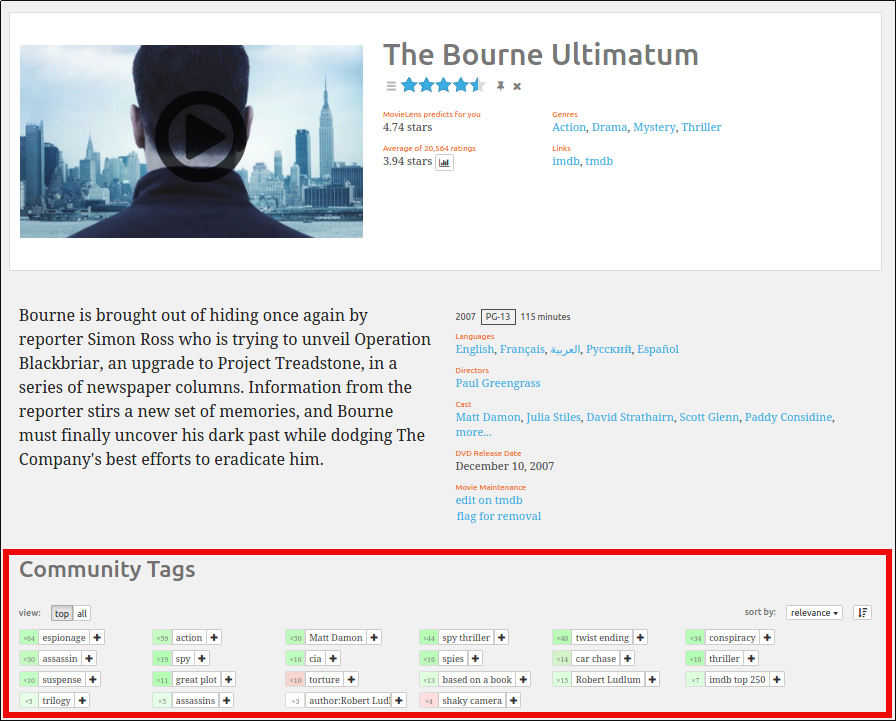
\includegraphics[width=\textwidth]{chapters/02_social_tagging/images/movielens.png}
    \caption{The MovieLens website supports tagging; any user can add their own tags and view tags assigned by other users to a particular resource. Retrieved from https://movielens.org/movies/54286 in January 2018.}
    \label{fig:movielens}
\end{figure}

\subsection{StackOverflow}

StackOverflow \footnote{https://stackoverflow.com/} is a very popular Q\&A (Question and Answer) website. It receives roughly 8,000 new questions related to computer programming every day. \footnote{As of 2017: https://stackoverflow.blog/2017/05/09/introducing-stack-overflow-trends/}

StackOverflow supports tagging of questions; users can add up to 5 tags to every question they post. Among other features, tags can be used to narrow down search results and they can also be subscribed to. Tags are also part of the website's incentive and reputation mechanisms; you can be awarded \textit{tag medals} for completing specific objectives such as answer many questions having a particular tag.

\begin{figure}[H]
    \centering
    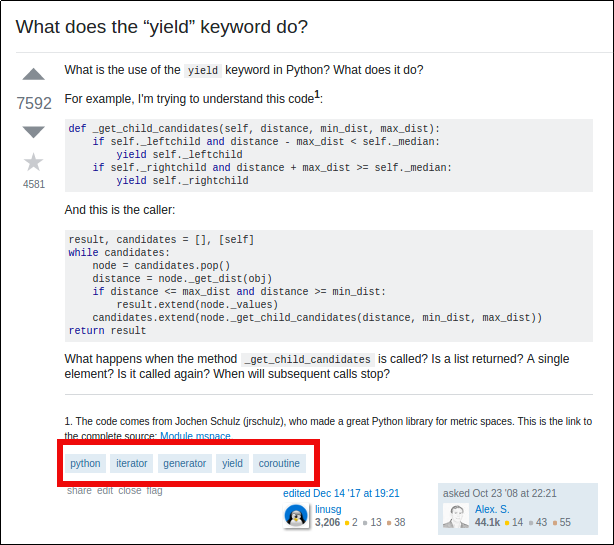
\includegraphics[width=\textwidth]{chapters/02_social_tagging/images/stackoverflow.png}
    \caption{The StackOverflow website also supports tagging, but only a single set of tags is shown, namely the tags assigned by the resource's original owner (and maybe edited afterwards). Retrieved from https://stackoverflow.com/questions/231767/what-does-the-yield-keyword-do in January 2018. }
    \label{fig:stackoverflow}
\end{figure}

\begin{figure}[H]
    \centering
    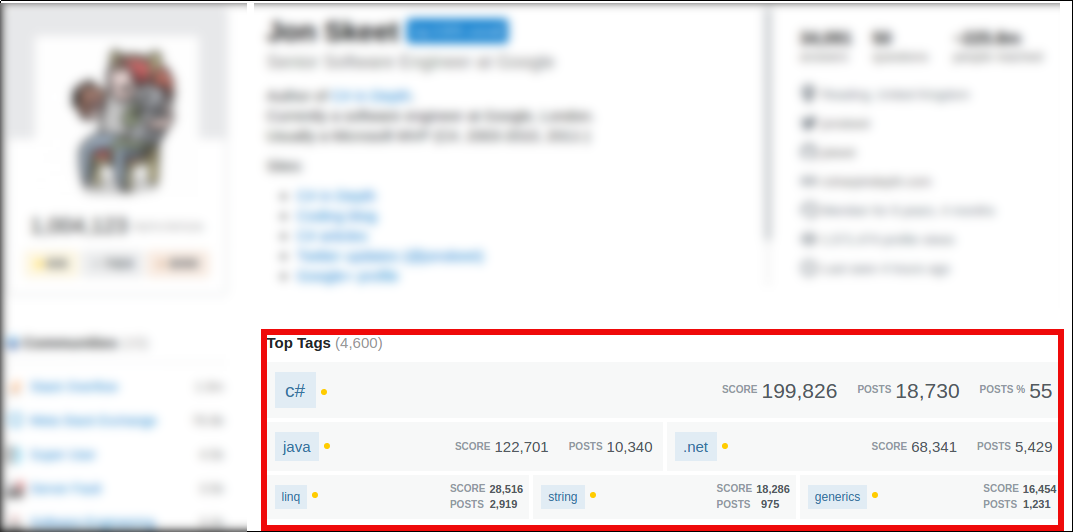
\includegraphics[width=\textwidth]{chapters/02_social_tagging/images/jon_skeet.png}
    \caption{Tags are also used to help drive Stackoverflow's incentive mechanisms; tag medals are awarded for activity related to a certain tag. Retrieved in January 2018. (Blur is used to protect the user's privacy)}
    \label{fig:jon_skeet}
\end{figure}

\section{Social Tagging and Folksonomies}

Since the beginning of STSs, it has been observed that such systems grow in an organic way and that certain patterns are noticed with respect to how tags are used. As an example, it has been observed \citep{halpin_etal_2006} that the number of times each tag is used to tag a particular resource forms a \textit{power law}, i.e. some tags are used exponentially more often than others.

More generally, the term \textbf{folksonomy} has been used to describe  these emerging patterns of informal organization and meaning assumed by tags in a Social Tagging System \citep{mathes_2004,wal_2005_folksonomy}.

According to \cite{mika_2007}, one way to model folksonomies is via \textit{tripartite hypergraphs}. Hypergraphs are generalizations of graphs \citep{berge_1985} where edges can join not just two but multiple nodes. Furthermore, hypergraphs representing folksonomies are also tripartite, inasmuch as there is a three-way \textit{partitioning} scheme (namely users-resources-tags) such that edges do not connect nodes that are in the same partition:

\begin{figure}[H]
    \begin{subfigure}{0.5\textwidth}
        \centering
    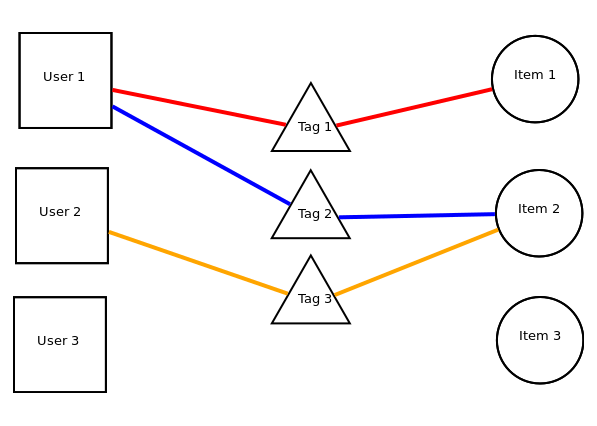
\includegraphics[width=0.8\textwidth]{chapters/02_social_tagging/images/folksonomy-hypergraph.png}
    \caption{User1-Tag1-Item1 (in red) is a single \textit{hyperedge} in this folksonomy hypergraph.}
    \label{fig:folksonomy_hypergraph}
    \end{subfigure}
    \begin{subfigure}{0.5\textwidth}
        \centering
    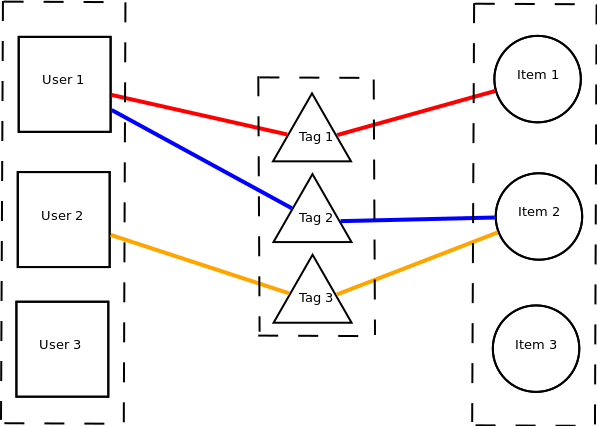
\includegraphics[width=0.8\textwidth]{chapters/02_social_tagging/images/tripartite.png}
    \caption{This is a \textit{tripartite} hypergraph because we can find 3 disjoint partitions}
    \label{fig:folksonomy_tripartite}
    \end{subfigure}
    \caption{A folksonomy can be represented as a tripartite hypergraph, where three-way hyperedges connect users, tags and items. Adapted from \cite{rawashdeh_etal_2012}. (Best viewed in colour).}
\end{figure}

The word \textit{folksonomy} itself (formed by \textit{folk} + \textit{taxonomy}) points to the fact that, differently from a rigid, often expert-driven taxonomy, the patterns that arise with the free use of tags by a community follows a more fluid, hapzard fashion, as can be  visualized in the next image where the the tag \textit{afghanistan} was used as search criterium on a photo-sharing website: 

\begin{figure}[H]
    \centering
    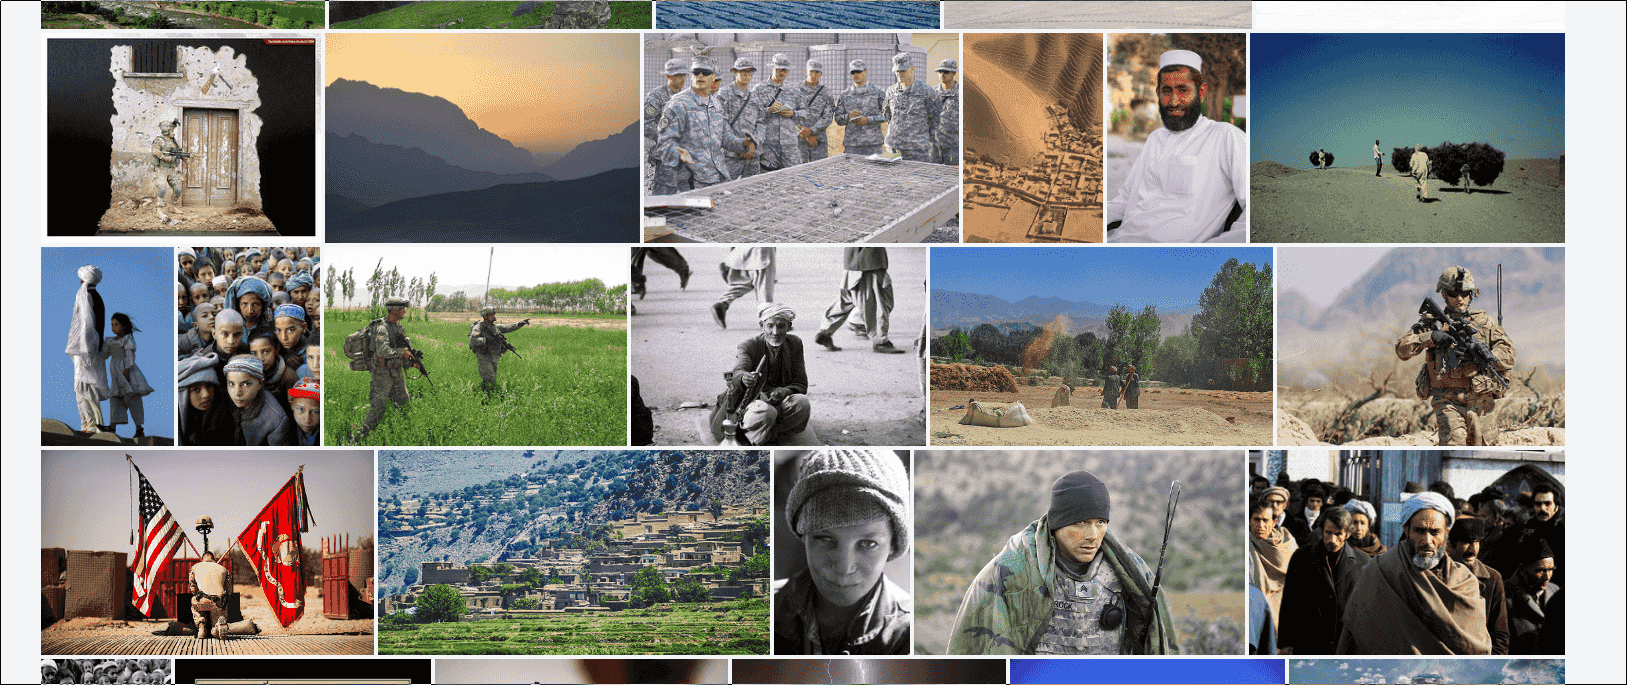
\includegraphics[width=\textwidth]{chapters/02_social_tagging/images/flickr_afghanistan.png}
    \caption{Searching for images tagged \textit{afghanistan} on Flickr yields pictures from the Afghani people, the war in Afghanistan, the Afghani landscape, etc. This reflects the multitude of meanings a single tag may acquire due to the way users tag their pictures. Retrieved from https://www.flickr.com/search/?tags=afghanistan in January 2018.}
    \label{fig:afghanistan}
\end{figure}

\section{Narrow and Broad Folksonomies}

Based on the examples given and one's general day-to-day experience, it's natural to conclude that folksonomies and their underlying STSs vary widely with respect to their features and how they're implemented.

One basic difference, raised as early as 2005 \citep{wal_2005_broad_and_narrow} and commented on by other authors \citep{marlow_etal_2006,halpin_etal_2006,peters_2009} since, is that between \textit{narrow} and \textit{broad} folksonomies.

\textbf{Narrow} folksonomies are folksonomies which only allow a resource's original poster (commonly referred to as \textit{O.P.} in such systems) to add tags to that resource. In other words, \textit{users can only tag their own content}.

Conversely, \textbf{broad} folksonomies are those where every user can add tags to any resource on the platform.

This distinction is relevant for researchers studying the dynamics of social tagging systems. For example, it has been noted by \cite{schifanella_etal_2010} that a global, shared tag vocabulary cannot be observed in narrow folksonomies, unless it is specifically promoted by the system.

On a similar note, \cite{aiello_2012} have suggested that tag predicting is more meaningful in broad folksonomies, since users can tag the same, global, set of resources. Also, tagging in such systems tend to reflect resource contents rather than users' personal preferences.

As related to the ease of navigation in STSs, \cite{helic_etal_2012} have suggested that broad folksonomies are better and more efficient for user browsing, inasmuch as these tags encode more information than their counterparts in narrow systems.

\section{Other Aspects}

Here we will talk about a few other aspects which we deem relevant in light of this work's objective, namely that of predicting tags in STSs.

\subsection{Tag Stabilization and Convergence}

In broad folksonomies (i.e. those where all users can add tags to any resource), the tag distribution for a given resource has been observed to stabilize after about 100 individual tag assignments \citep{golder_huberman_2006}. Reasons given for this phenomenon include \textit{imitation}, i.e. users are influenced by other tags already given to a resource and \textit{shared knowledge}, i.e. other tags help build a user's mental model of the meaning for each tag.

We consider this an important result because it may affect the level of tag prediction we can achieve. One can view it graphically in the following image:

\begin{figure}[H]
    \centering
    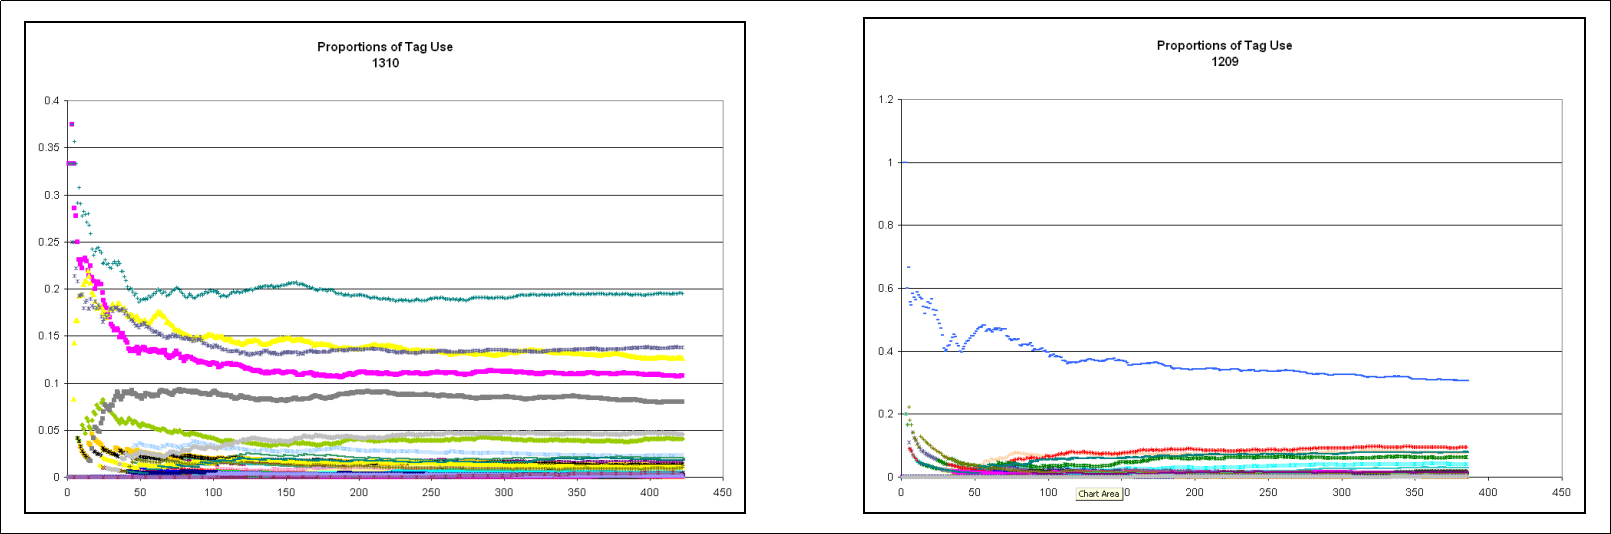
\includegraphics[width=\textwidth]{chapters/02_social_tagging/images/golder_huberman.png}
    \caption{Tag distributions for two resources on Delicious.com. Tag proportions reach equilibrium after around 100 tag assignments. Adapted from \cite{golder_huberman_2005}}
    \label{fig:golder_huberman}
\end{figure}

\subsection{Effect of tag suggestion on STSs}

It has been suggested by \cite{marlow_etal_2006} that a STS falls under one of three types depending upon how much system support there is for tagging:

\begin{itemize}[noitemsep]
\item \textit{Blind Tagging}: Users cannot view other tags assigned to an item, before adding their own.
\item \textit{Viewable Tagging}: Users can view other tags assigned to an item before adding their own tags.
\item \textit{Suggestive Tagging}: Users can not only view other tags but the system also suggests appropriate tags.\citep{marlow_etal_2006}
\end{itemize}

They have suggested that the level of tagging support (as referred to above) present in a system may make tag stabilization and convergence faster.

In light of that, we can suggest that tag prediction can contribute to a higher quality STS, if we assume that a folksonomy where the global vocabulary has converged is more useful than one where it hasn't.


